%%%%%%%%%%%%%%%%%%%%%%%%%%%%% Define Article %%%%%%%%%%%%%%%%%%%%%%%%%%%%%%%%%%
\documentclass{article}
%%%%%%%%%%%%%%%%%%%%%%%%%%%%%%%%%%%%%%%%%%%%%%%%%%%%%%%%%%%%%%%%%%%%%%%%%%%%%%%
%%%%%%%%%%%%%%%%%%%%%%%%%%%%% Using Packages %%%%%%%%%%%%%%%%%%%%%%%%%%%%%%%%%%
\usepackage{geometry}
\usepackage{graphicx}
\usepackage{amssymb}
\usepackage{amsmath}
\usepackage{amsthm}
\usepackage{empheq}
\usepackage{mdframed}
\usepackage{booktabs}
\usepackage{lipsum}
\usepackage{graphicx}
\usepackage{color}
% \usepackage{psfrag}
\usepackage{pgfplots}
\usepackage{bm}
\usepackage{amsmath}
\usepackage[most]{tcolorbox}
\usepackage{xparse}
\usepackage{darkmode}
\usepackage[stable]{footmisc}
\usepackage{gensymb}
\usepackage{siunitx}
\usepackage[colorlinks]{hyperref}
\usepackage{fancyhdr}
\usepackage{varwidth}


% --- Glossaries + TikZ externalization friendly setup ---
\makeatletter
\@ifundefined{pgfexternalrealjob}{%
  % Main document run: full glossaries with automake
  \usepackage[automake]{glossaries-extra}%
}{%
  % External TikZ runs: minimal glossaries that don't try to build/read files
  \usepackage[nostyles]{glossaries-extra}%
  % Pretend glossary files don't exist, so no "use \makeglossaries" error
  \def\glsifexists#1#2#3{#3}%
}
\makeatother

\usetikzlibrary{calc,decorations.pathreplacing, arrows.meta, positioning, external}


%%%%%%%%%%%%%%%%%%%%%%%%%%%%%%%%%%%%%%%%%%%%%%%%%%%%%%%%%%%%%%%%%%%%%%%%%%%%%%%

% Other Settings
\enabledarkmode

%%%%%%%%%%%%%%%%%%%%%%%%%% Page Setting %%%%%%%%%%%%%%%%%%%%%%%%%%%%%%%%%%%%%%%
\geometry{a4paper}

%%%%%%%%%%%%%%%%%%%%%%%%%% Define some useful colors %%%%%%%%%%%%%%%%%%%%%%%%%%
\definecolor{ocre}{RGB}{243,102,25}
\definecolor{mygray}{RGB}{243,243,244}
\definecolor{deepGreen}{RGB}{26,111,0}
\definecolor{shallowGreen}{RGB}{235,255,255}
\definecolor{deepBlue}{RGB}{61,124,222}
\definecolor{shallowBlue}{RGB}{235,249,255}
%%%%%%%%%%%%%%%%%%%%%%%%%%%%%%%%%%%%%%%%%%%%%%%%%%%%%%%%%%%%%%%%%%%%%%%%%%%%%%%

%%%%%%%%%%%%%%%%%%%%%%%%%% Define an orangebox command %%%%%%%%%%%%%%%%%%%%%%%%
\newcommand\orangebox[1]{\fcolorbox{ocre}{mygray}{\hspace{1em}#1\hspace{1em}}}
%%%%%%%%%%%%%%%%%%%%%%%%%%%%%%%%%%%%%%%%%%%%%%%%%%%%%%%%%%%%%%%%%%%%%%%%%%%%%%%

%%%%%%%%%%%%%%%%%%%%%%%%%%%% English Environments %%%%%%%%%%%%%%%%%%%%%%%%%%%%%

%%%%%%%%%%%%%%%%%%%%%%%%%%%%% Theorem Macro %%%%%%%%%%%%%%%%%%%%%%%%%%%%%%%%%%%
\newtheoremstyle{mytheoremstyle}{3pt}{3pt}{\normalfont}{0cm}{\rmfamily\bfseries}{}{1em}{{\color{black}\thmname{#1}~\thmnumber{#2}}\thmnote{\,--\,#3}}
\newtheoremstyle{myproblemstyle}{3pt}{3pt}{\normalfont}{0cm}{\rmfamily\bfseries}{}{1em}{{\color{white}\thmname{#1}~\thmnumber{#2}}\thmnote{\,--\,#3}}
\theoremstyle{mytheoremstyle}
\newmdtheoremenv[linewidth=1pt,backgroundcolor=shallowGreen,linecolor=deepGreen,leftmargin=0pt,innerleftmargin=20pt,innerrightmargin=20pt,]{theorem}{Theorem}[section]
\theoremstyle{mytheoremstyle}
\newmdtheoremenv[linewidth=1pt,backgroundcolor=shallowBlue,linecolor=deepBlue,leftmargin=0pt,innerleftmargin=20pt,innerrightmargin=20pt,]{definition}{Definition}[section]
\theoremstyle{myproblemstyle}
\newmdtheoremenv[linecolor=black,leftmargin=0pt,innerleftmargin=10pt,innerrightmargin=10pt,]{problem}{Problem}[section]
%%%%%%%%%%%%%%%%%%%%%%%%%%%%%%%%%%%%%%%%%%%%%%%%%%%%%%%%%%%%%%%%%%%%%%%%%%%%%%%


\theoremstyle{myproblemstyle}
\newmdtheoremenv[
        linewidth=1pt,
        backgroundcolor=black!85,
        fontcolor = white!90,
        linecolor=white!100,
        leftmargin=0pt,
        innerleftmargin=20pt,
        innerrightmargin=20pt,]{example}{Example}[section]



%%%%%%%%%%%%%%%%%%%%%%%%%%%%%%%%%%%%%%%%%%%%
%%%%%%%%%%%%%%% Equation Macro %%%%%%%%%%%%%
%%%%%%%%%%%%%%%%%%%%%%%%%%%%%%%%%%%%%%%%%%%%

% Simple mdframed style for equation boxes (no TikZ)
\newmdenv[
        linewidth=1pt,
        backgroundcolor=black!85,
        fontcolor = white!90,
        linecolor=white!100,
        leftmargin=0pt,
        innerleftmargin=20pt,
        innerrightmargin=20pt,]
        {eqbox}

\ExplSyntaxOn
\seq_new:N \g_piers_eq_seq

% Store (label, title, equation-body) for later printing
\cs_new_protected:Npn \piers_add_eq:nnn #1#2#3
  {
    \seq_gput_right:Nn \g_piers_eq_seq
      { \piers_eq_entry:nnn {#1}{#2}{#3} }
  }

% How each equation is printed in the final summary
\cs_new_protected:Npn \piers_eq_entry:nnn #1#2#3
  {
    \par\noindent
    \begin{minipage}{0.72\linewidth}
      \begin{equation*}
        #3
      \end{equation*}
    \end{minipage}
    \begin{minipage}{0.9\linewidth}
      \raggedright
      \qquad\eqref{#1}\;(\textit{#2})
    \end{minipage}

    \par\bigskip
  }

% Environment: \begin{eqboxed}{label}{Title}{Description} <equation> \end{eqboxed}
\NewDocumentEnvironment{eqboxed}{ m m m +b }
  {
    % begin code: mdframed-based, no TikZ
    \begin{eqbox}
      {\bfseries #2}\par\vspace{0.4em}%
      \begin{equation}
        \label{#1}
        #4
      \end{equation}
      #3
    \end{eqbox}
    % store equation body for later
    \piers_add_eq:nnn{#1}{#2}{#4}
  }
  {
    % end code
  }

% Command to print all stored equations at the end
\NewDocumentCommand{\PrintAllEquations}{}
  {
    \section{Equations}
    \seq_use:Nn \g_piers_eq_seq { }
  }
\ExplSyntaxOff

% ----------------------------
% Constants boxed environment
% ----------------------------
\newmdenv[
  framemethod=default,
  linewidth=1pt,
  backgroundcolor=black!85,
  fontcolor = white!90,
  linecolor=white!100,
  leftmargin=0pt,
  innerleftmargin=20pt,
  innerrightmargin=20pt,
]{constbox}

\ExplSyntaxOn
\seq_new:N \g_piers_const_seq

% Store (label, title, constant-body) for later printing
\cs_new_protected:Npn \piers_add_const:nnn #1#2#3
  {
    \seq_gput_right:Nn \g_piers_const_seq
      { \piers_const_entry:nnn {#1}{#2}{#3} }
  }

% How each constant is printed in the final summary
\cs_new_protected:Npn \piers_const_entry:nnn #1#2#3
  {
    \par\noindent
    \begin{minipage}{0.72\linewidth}
      % mirror your equation* block, but as display math
      \[
        #3
      \]
    \end{minipage}
    \begin{minipage}{0.9\linewidth}
      \raggedright
      \qquad(\texttt{\ref{#1}})\;(\textit{#2})
    \end{minipage}

    \par\bigskip
  }

\newcounter{const}
\renewcommand{\theconst}{\arabic{const}}

% Environment: \begin{constboxed}{label}{Title}{Description} <constant> \end{constboxed}
\NewDocumentEnvironment{constboxed}{ m m m +b }
  {
    \refstepcounter{const}
    \begin{constbox}
      {\bfseries #2}\par\vspace{0.4em}%
      \label{#1}
      \[ 
        #4
      \]
      #3
    \end{constbox}
    % store constant body for later
    \piers_add_const:nnn{#1}{#2}{#4}
  }
  {}

% Command to print all stored constants at the end
\NewDocumentCommand{\PrintAllConstants}{}
  {
    \section{Constants}
    \seq_use:Nn \g_piers_const_seq { }
  }
\ExplSyntaxOff






%%%%%%%%%%%%%%%%%%%%%%%%%%%%%%% Plotting Settings %%%%%%%%%%%%%%%%%%%%%%%%%%%%%
\usepgfplotslibrary{colorbrewer}
\pgfplotsset{width=8cm,compat=1.9}
%%%%%%%%%%%%%%%%%%%%%%%%%%%%%%%%%%%%%%%%%%%%%%%%%%%%%%%%%%%%%%%%%%%%%%%%%%%%%%%

%%%%%%%%%%%%%%%%%%%%%%%%%%%%%%% Title & Author %%%%%%%%%%%%%%%%%%%%%%%%%%%%%%%%
\title{Notes}
\author{Pierson Lipschultz}
%%%%%%%%%%%%%%%%%%%%%%%%%%%%%%%%%%%%%%%%%%%%%%%%%%%%%%%%%%%%%%%%%%%%%%%%%%%%%%%

%%%%%%%%%%%%%%%%%%%%%%% Glossary entries %%%%%%%%%%%%%%%%%%%%%%%%%%%%%%%%%%%%%%

\newglossaryentry{test}{
name={test},
description={test}
}
% Only do the real glossaries work in the main document run
\tikzifexternalizing{}{%
  \makeglossaries
}

% \tikzexternalize[prefix=tikz-cache/]
%%%%%%%5%%%%%%%%%%%%%%%%%%%55
\begin{document}
    \pagestyle{fancy}

    \fancyhf{}
    \fancyfoot[L]{\nouppercase{\leftmark}} % "1 INTRODUCTION"
    \fancyfoot[R]{\thepage}% page number on right

    % Remove header rule and add footer rule instead
    \renewcommand{\headrulewidth}{0pt}
    \renewcommand{\footrulewidth}{0.4pt}
    \renewcommand{\sectionmark}[1]{\markboth{#1}{}}

    \maketitle
    \tableofcontents

    \section{Coulomb's Law}
    \begin{eqboxed}{eq:CoulombsLaw}{Coulomb's Law}
    {Gives a force along the line of two charges. \\ If \(q_1\) and \(q_2\) have the same sign (i.e. charge) then the force must be repulsive. But if they have the \textit{same} sign, then it must be attractive.\\ 
    Because of Newton's second law, \(F_{12} = -F_{21}\)}
    \vec{F_{12}} =k\frac{q_1q_2}{r_{12}^2}\hat{r_{12}} 
    \end{eqboxed}

\begin{center}
  % \boxed{\vec{F_{12}} =k\frac{q_1q_2}{r_{12}^2}\hat{r_{12}}}
  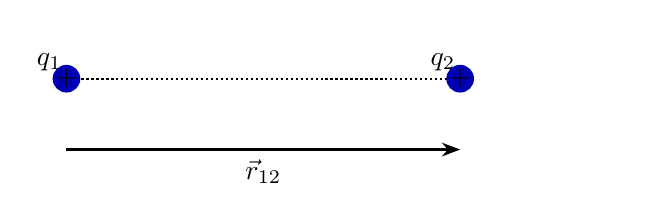
\begin{tikzpicture}[>=Stealth, thick]
    % --- Positions ---
    \coordinate (q1) at (0,0);
    \coordinate (q2) at (5,0);
  
    % --- Dotted separation line ---
    \draw[densely dotted] (q1) -- (q2);
  
    % --- Charges as filled circles ---
    \fill[blue!70!black] (q1) circle (5pt);

  
    % --- Labels for charges ---
    \node[above left=-1pt and -2pt] at (q1) {$q_1$};
    \node[above left=-1pt and -2pt] at (q2) {$q_2$};
    \node[] at (q1) {$+$};

  
    % --- Force arrow from q2 to the right ---
    \draw[white, very thick, ->] (q2) -- ++(2.2,0)
      node[midway, above] {$\vec{F}_{12}$};

    \fill[blue!70!black] (q2) circle (5pt);
    \node[] at (q2) {$+$};

    % --- r_12 arrow below ---
    \draw[->] ($(q1)+(0,-0.9)$) -- ($(q2)+(0,-0.9)$)
      node[midway, below] {$\vec{r}_{12}$};
  \end{tikzpicture}

    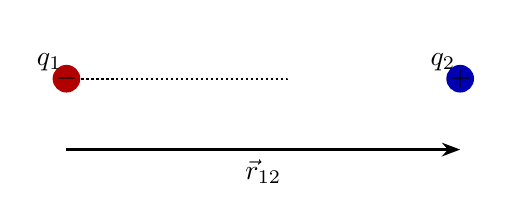
\begin{tikzpicture}[>=Stealth, thick]
    % --- Positions ---
    \coordinate (q1) at (0,0);
    \coordinate (q2) at (5,0);
  
    % --- Dotted separation line ---
    \draw[densely dotted] (q1) -- (q2);
  
    % --- Charges as filled circles ---
    \fill[red!70!black] (q1) circle (5pt);

  
    % --- Labels for charges ---
    \node[above left=-1pt and -2pt] at (q1) {$q_1$};
    \node[above left=-1pt and -2pt] at (q2) {$q_2$};
    \node[] at (q1) {$-$};

  
    % --- Force arrow from q2 to the right ---
    \draw[white, very thick, ->] (q2) -- ++(-2.2,0)
      node[midway, above] {$\vec{F}_{12}$};

    \fill[blue!70!black] (q2) circle (5pt);
    \node[] at (q2) {$+$};

    % --- r_12 arrow below ---
    \draw[->] ($(q1)+(0,-0.9)$) -- ($(q2)+(0,-0.9)$)
      node[midway, below] {$\vec{r}_{12}$};
  \end{tikzpicture}

  \pagebreak

  \boxed{F_{1,net} = F_{21} + F_{31}}

  \begin{tikzpicture}[>=Stealth, thick]
    % --- Positions ---
    \coordinate (q1) at (0,0);
    \coordinate (q2) at (5,0);
    \coordinate (q3) at (0,-5);
  
    % --- Dotted separation line ---
    \draw[densely dotted] (q1) -- (q2);
    \draw[densely dotted] (q1) -- (q3);
  
    % --- Charges as filled circles ---


    \draw[white, very thick, ->] (q1) -- ++(2.2,0)
      node[midway, above] {$\vec{F}_{21}$};

    \draw[white, very thick, ->] (q1) -- ++(0,-2.2)
      node[midway, left] {$\vec{F}_{31}$};

    \draw[white, very thick, ->] (q1) -- ++(2,-2)
      node[midway, left] {$\vec{F}_{net}$};

    \fill[blue!70!black] (q1) circle (5pt);

    % --- Labels for charges ---
    \node[above left] at (q1) {$q_1$};
    \node[below right] at (q2) {$q_2$};
    \node[below right] at (q3) {$q_3$};
    \node[] at (q1) {$-$};

  
    % --- Force arrow from q2 to the right ---
    % \draw[white, very thick, ->] (q2) -- ++(-2.2,0)
    %   node[midway, above] {$\vec{F}_{12}$};

    %       % --- Force arrow from q2 to the right ---
    % \draw[white, very thick, ->] (q3) -- ++(0,2.2)
    %   node[midway, right] {$\vec{F}_{13}$};


    \fill[red!70!black] (q2) circle (5pt);
    \node[] at (q2) {$+$};

    \fill[red!70!black] (q3) circle (5pt);
    \node[] at (q3) {$+$};


    % % --- r_12 arrow below ---
    % \draw[->] ($(q1)+(0,-0.9)$) -- ($(q2)+(0,-0.9)$)
    %   node[midway, below] {$\vec{r}_{12}$};
  \end{tikzpicture}

\end{center}

\begin{eqboxed}{eq:SuperpostionPrinciple}{Superpostion Principle}
{}
F_{net} = \sum_i \vec{F_i}
\end{eqboxed}
\begin{constboxed}{const:e}{Electron Charge}
{}
e = -1.6 \times 10^{-19} C
\end{constboxed}

\begin{constboxed}{const:k}{k}
{}
k = 9 \times 10^9 \frac{NM^2}{C^2}
\end{constboxed}


\pagebreak
\subsection{Examples}
\hrule
\vspace{.5cm}


\begin{example}

\begin{center} 
  \boxed{F_{3,net}= ???}\vspace{.5cm}
      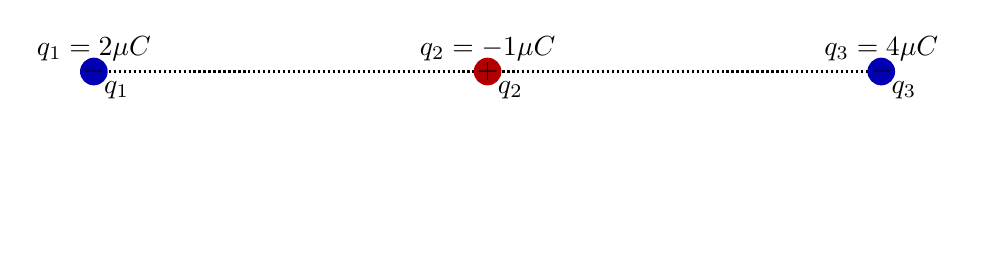
\begin{tikzpicture}[>=Stealth, thick]
      % --- Positions ---
      \coordinate (q1) at (-5,0);
      \coordinate (q2) at (0,0);
      \coordinate (q3) at (5,0);
    
      % --- Dotted separation line ---
      \draw[densely dotted] (q1) -- (q2);
      \draw[densely dotted] (q1) -- (q3);
    
      % --- Charges as filled circles ---
      
      \draw[white, very thick, <->] ($(q1) +(0,-1.5)$) -- ($(q2) +(-.2,-1.5)$)
        node[midway, below] {$1m$};

      \draw[white, very thick, <->] ($(q2) +(+.2,-1.5)$) -- ($(q3) +(0,-1.5)$)
        node[midway, below] {$1m$};

  
      \draw[white, very thick, ->] ($(q3) +(0,-.4)$) -- ++(1.2,0)
        node[midway, below] {$\vec{F}_{13}$};
  
  
      \draw[white, very thick, ->] ($(q3) +(0,-.5)$) -- ++(-2.2,0)
        node[midway, below] {$\vec{F}_{23}$};
  
      \fill[blue!70!black] (q1) circle (5pt);
      \node[] at (q1) {$-$};

      % --- Labels for charges ---
      \node[below right] at (q1) {$q_1$};
      \node[below right] at (q2) {$q_2$};
      \node[below right] at (q3) {$q_3$};

      \node[above] at (q1) {$q_1 = 2  \mu C$};
      \node[above] at (q2) {$q_2 = -1 \mu C$};
      \node[above] at (q3) {$q_3 = 4  \mu C$};
  
    
      % --- Force arrow from q2 to the right ---
      % \draw[white, very thick, ->] (q2) -- ++(-2.2,0)
      %   node[midway, above] {$\vec{F}_{12}$};
  
      %       % --- Force arrow from q2 to the right ---
      % \draw[white, very thick, ->] (q3) -- ++(0,2.2)
      %   node[midway, right] {$\vec{F}_{13}$};
  
  
      \fill[red!70!black] (q2) circle (5pt);
      \node[] at (q2) {$+$};
  
      \fill[blue!70!black] (q3) circle (5pt);
      \node[] at (q3) {$-$};
  
  
      % % --- r_12 arrow below ---
      % \draw[->] ($(q1)+(0,-0.9)$) -- ($(q2)+(0,-0.9)$)
      %   node[midway, below] {$\vec{r}_{12}$};
      \end{tikzpicture}
\end{center}

\hrule
\vspace{.5cm}
Using Coulomb's Law\ref{eq:CoulombsLaw}\dots
\[
\vec{F_{3,net}} = \vec{F_{31}} + \vec{F_{32}} \]
\[\vec{F_{31}} = k \frac{q_3q_1}{r_{31}^2} \hat{r_{32}}\]
\[\vec{F_{32}} = k \frac{q_3q_2}{r_{32}^2} \hat{r_{32}}\]
\[k = 9 \times 10^9 \frac{NM^2}{C^2},  \qquad q_1 = 2\mu C, \qquad q_2 = -1 \mu C, \qquad q_3 = 4\mu C \]
\[\vec{F_{31}} = \SI{1.800e-02}{\N}, \quad \vec{F_{32}} = \SI{-3.600e-02}{\N}\]
\[\boxed{\vec{F}_{3, net} =  \SI{-1.800e-02}{\N}}\]
\end{example}


    
\pagebreak
\PrintAllEquations
\PrintAllConstants
\tikzifexternalizing{}{%
  \printglossaries
}

\end{document}
